% THIS IS SIGPROC-SP.TEX - VERSION 3.1
% WORKS WITH V3.2SP OF ACM_PROC_ARTICLE-SP.CLS
% APRIL 2009
%
% It is an example file showing how to use the 'acm_proc_article-sp.cls' V3.2SP
% LaTeX2e document class file for Conference Proceedings submissions.
% ----------------------------------------------------------------------------------------------------------------
% This .tex file (and associated .cls V3.2SP) *DOES NOT* produce:
%       1) The Permission Statement
%       2) The Conference (location) Info information
%       3) The Copyright Line with ACM data
%       4) Page numbering
% ---------------------------------------------------------------------------------------------------------------
% It is an example which *does* use the .bib file (from which the .bbl file
% is produced).
% REMEMBER HOWEVER: After having produced the .bbl file,
% and prior to final submission,
% you need to 'insert'  your .bbl file into your source .tex file so as to provide
% ONE 'self-contained' source file.
%
% Questions regarding SIGS should be sent to
% Adrienne Griscti ---> griscti@acm.org
%
% Questions/suggestions regarding the guidelines, .tex and .cls files, etc. to
% Gerald Murray ---> murray@hq.acm.org
%
% For tracking purposes - this is V3.1SP - APRIL 2009

\documentclass{acm_proc_article-sp}
\usepackage{graphicx}

\makeatletter
\def\@copyrightspace{\relax}
\makeatother

\begin{document}

\title{MichelinCook - an easy way to cook better}
%\subtitle{[Extended Abstract]}
%
% You need the command \numberofauthors to handle the 'placement
% and alignment' of the authors beneath the title.
%
% For aesthetic reasons, we recommend 'three authors at a time'
% i.e. three 'name/affiliation blocks' be placed beneath the title.
%
% NOTE: You are NOT restricted in how many 'rows' of
% "name/affiliations" may appear. We just ask that you restrict
% the number of 'columns' to three.
%
% Because of the available 'opening page real-estate'
% we ask you to refrain from putting more than six authors
% (two rows with three columns) beneath the article title.
% More than six makes the first-page appear very cluttered indeed.
%
% Use the \alignauthor commands to handle the names
% and affiliations for an 'aesthetic maximum' of six authors.
% Add names, affiliations, addresses for
% the seventh etc. author(s) as the argument for the
% \additionalauthors command.
% These 'additional authors' will be output/set for you
% without further effort on your part as the last section in
% the body of your article BEFORE References or any Appendices.

\numberofauthors{5} %  in this sample file, there are a *total*
% of EIGHT authors. SIX appear on the 'first-page' (for formatting
% reasons) and the remaining two appear in the \additionalauthors section.
%
\author{
% You can go ahead and credit any number of authors here,
% e.g. one 'row of three' or two rows (consisting of one row of three
% and a second row of one, two or three).
%
% The command \alignauthor (no curly braces needed) should
% precede each author name, affiliation/snail-mail address and
% e-mail address. Additionally, tag each line of
% affiliation/address with \affaddr, and tag the
% e-mail address with \email.
%
% 1st. author
\alignauthor
Pratheek L K Murthy\\
       \affaddr{Department of Electrical and Computer Engineering}\\
       \affaddr{Texas A\&M University}\\
% 2nd. author
\alignauthor
Srinath Nadimpalli\\
		\affaddr{Department of Computer Science and Engineering}\\
		\affaddr{Texas A\&M University}\\
% 3rd. author
\alignauthor
Sri Jeevanige\\
		\affaddr{Department of Computer Science and Engineering}\\
		\affaddr{Texas A\&M University}\\
\and  % use '\and' if you need 'another row' of author names
% 4th. author
\alignauthor 
Smit Shah\\
	\affaddr{Department of Computer Science and Engineering}\\
	\affaddr{Texas A\&M University}\\
% 5th. author
\alignauthor 
Xiaoguang Ma\\
\affaddr{Department of Civil Engineering}\\
\affaddr{Texas A\&M University}\\
}


\maketitle
\begin{abstract}
In this paper, we describe a novel method for delivering cooking instructions in the form of self-timed digital cards. We will discuss the shortcomings of current available methods for providing cooking instructions to the user. The merits of self-timed timed digital cards presented in the mobile application MichelinCook is then discussed. We will then discuss the design and implementation of MichelinCook as an android application. The paper also describes the design of hardware system for controlling the temperature of cook-top and integrating it with the mobile application. Finally we discuss the evaluation methods for the system and about the scope for future work.  
\end{abstract}

% A category with the (minimum) three required fields
%\category{H.4}{Information Systems Applications}{Miscellaneous}
%%A category including the fourth, optional field follows...
%\category{D.2.8}{Software Engineering}{Metrics}[complexity measures, performance measures]

%\terms{Theory}

\keywords{Self-time digital cards, recipe delivery, mobile application, temperature control} % NOT required for Proceedings

\section{Introduction} 
The kitchen plays an important emotional role in our lives. Everyone enjoys getting together with friends or family for meals, especially during festivals or holidays. These celebrations are usually potluck in nature and it would be awkward to bring in off the shelf food for such meet-ups. Moreover, it is believed widely that ''The easiest way to Man's heart is through his stomach'', making it more important to cook for you loved ones. It also becomes essential to cook your own meal when you are on a particular diet or want to have a healthier lifestyle. So it is no exaggeration to say that ability to cook improves your life greatly.

But there are many people who do not take to cooking because of the fear that manifests from this exercise. Some people are overwhelmed by the recipes which may be complicated to cook from or overly long and fear missing the steps, some are intimidated by the cooking techniques involved because of not clearly understanding them, some fear that they may overcook the food, some fear seasoning the food wrongly and there are some others who worry about how the food looks. This phobia or fear of cooking is termed as Mageirocophobia.

However we believe that it is possible to alleviate the above mentioned fear by providing an easy and intuitive user interface to deliver the cooking instructions.

\section{Problem Statement}
The current available system for delivery of cooking instructions is difficult to follow and confusing to cook from. We did a survey to find out what are the different medias that people use to cook from and found out that people use recipe blogs, YouTube videos, paperback recipe books, recipe apps etc.., 

There are several shortcomings of using the above listed medias for cooking. The conventional paperback and recipe blogs are difficult to cook from because of them being static and less intuitive. Using YouTube videos during cooking is cumbersome as it is difficult when trying to refer to a previous step and results in a lot of pause, rewind and forward. The current available apps provides solution to many of the above mentioned problems but we believe that the cooking experience can be further enhanced by feature set of MichelinCook.

Our mobile application mainly aims at providing the user with cooking instructions in the form of self-timed digital cards \cite{CardView}. Flash Cards have been used as an effective strategy for studying, we use a modified version of the flash cards to make up the cards used to provide the cooking directions. The cooking procedure is broken down into many steps and each card presents an individual step with a timer(which runs down from the required time for that step). The important steps are additionally presented with photographs on the cards and can be used as references to further enhance the cooking process.
\section{Design}
The design goal of MichelinCook is to provide timing based delivery of flash cards containing cooking directions. Following are the important design goals of the application.

\begin{enumerate}
	\item Easy search and access to Recipes
	\item Access to latest trending recipes and curated recipes from popular chefs
	\item Finding recipes based on categories like 'Cuisines, 'Quick \& Easy', 'Cheap Eats' and 'Healthy'
	\item Direct search for a recipe from every page
	\item Easy navigation throughout the app
	
\end{enumerate}

\begin{itemize}
\item Interactive content delivery for cooking
\item Table of required quantity of ingredients for selected recipe
\item The quantity of ingredients are appropriately changed depending on the number of servings selected
\item Cook-top size is considered to scale the time required for each cooking step
\item Timer enabled flash cards containing cooking direction and picture to assist while cooking
\item Ability to navigate to any step of the cooking procedure
\end{itemize}

The above listed features will help provide user with an easy and direct way to cook from. The overall experience is further enhanced by a simple UI design.

\section{Social and Cognitive Issues}
It should go without saying that smartphones make our lives easier in many ways. They help us find directions to our next destination, maintain communication with loved ones and dear friends, and even waste precious time playing games. We carry our phones with us everywhere we go, be it our living room, work space, or even the bathroom. So why shouldn't we venture with it into the kitchen? Cooking apps are the next step in the complete mobile takeover.

The app revolution is leaving no sphere of life untouched, not even the kitchen. With more devices featuring large and vivid touch screens, it is trivial to realize that a good tablet with the right apps can make for a handy digital cookbook, able to help home cooks and pro chefs discover and organize recipes, track shopping lists and organize menus and meal calendars. From recipe discovery apps and classic cookbooks, to personal recipe organizers, there are now apps for Android, iOS, Windows Phone and Windows 8 devices.

But with MichelinCook user experiences features that are clear and concise. The digital cards provides a unique solution to enable users to cook a variety of dishes. The digital cards are designed for ease of learning, with step-by-step instructions, allowing users to see exactly what's going on all the time.
\section{Implementation} 

\subsection{Step 1 : Application Workflow and UI Design}
	
The application was conceptualized and prototyped using Justinmind Prototyper. 

Initially we did the UI design of the application in JustinMind tool. 
When we launch the Android application, Screen shown in Figure 1 will be shown in the app which we call the Main screen. The rationale behind the UI design of this first screen is to show the user all the top recipes to get their attention. 
Now the user can click the Navigation drawer panel at the top left corner of the screen.
Following which all the recipe categories such as Cheap Eats,Healthy recipes, Quick and Easy recipes and Cuisines will be shown on the left fragment view of the screen. 
The rationale behind providing these recipe categories are users often tend to find search functionality to search for appropriate recipes by keyword search based mechanism. 
By having the popular dishes and more frequently used recipe categories, we are offering users easy way of accessing and finding their recipes and showing an element of surprise.
The reason behind choosing the Healthy recipes as recipe category is that users who are on a diet plan can easily find the list of healthy recipes with our application instead of searching for a recipe and later figuring out if that recipe is healthy or not.The reason behind choosing the Cheap Eats recipe is for cooks who are trying to save money and on a budget plan, we will show the recipes that are cheap. 
Similarly, we have provided Quick and Easy recipe category for the cooks who are running out of time and in a hurry to make some dish. 

Once the cook selects one of the recipe categories, any one of the screens in the figures 3,4,5,6 will be shown in the app. 
Now, the cook can select any one of the recipes listed on the screen. As they do that, the recipe review screen, as shown in Figure 7 will be launched. The recipe review screen displays the image of the recipe, list of ingredient and their quantities required to prepare the dish. Now, the cook can review the ingredients and check if they have it or need to buy them from groceries. When the cook decides to prepare the dish, he will collect all the ingredients listed in the recipe review screen and press 'Cook' button.

Now, the user sees the recipe cards screen as shown in Figure 8. This screen lists out all the steps of the cooking process. Each recipe card shows a step in the cooking process. Each recipe card consists of cooking directions, time needed for that step and the image describing the step. 

So, the users can scroll down the screen seeing one card at a time on the screen. When they click the start button at the top, timer keeps ticking down until it reaches to zero. On reaching zero, the app automatically scrolls down to the recipe card of the next step.This enables the user to concentrate fully on his cooking.

We also added functionality to 'Pause' the timer in cases when the user has to leave the kitchen. When the user clicks the 'Pause' button, the timer is paused. The user clicks the 'Resume' button again as shown in Figure 9. So, using this application, user can have smooth cooking experience.

\begin{figure}[ht!]
	\centering
	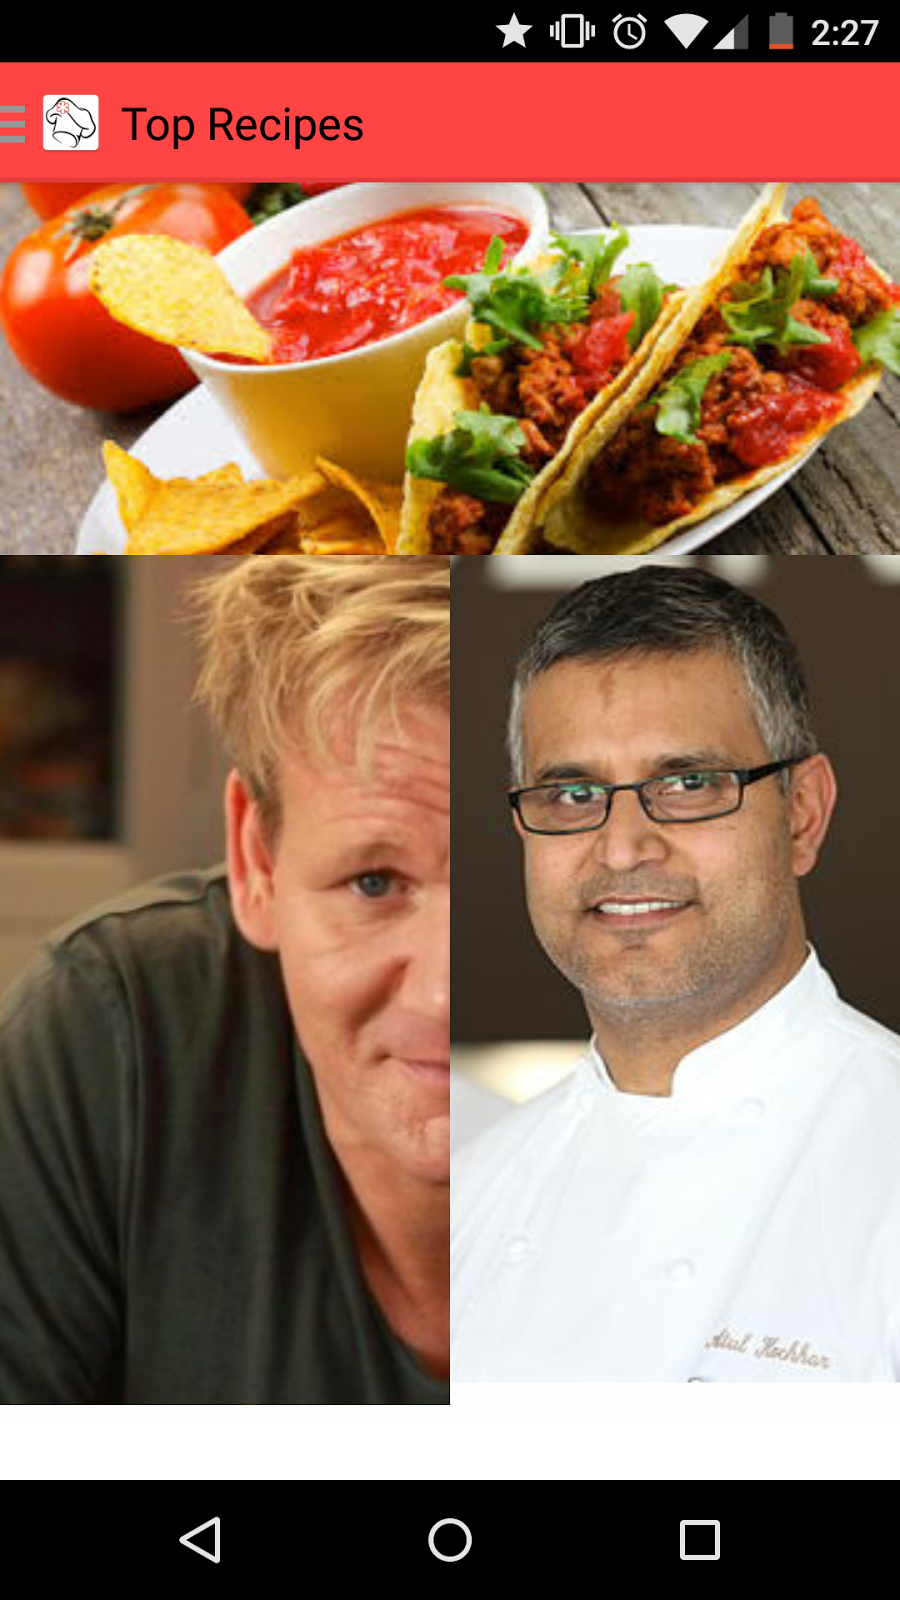
\includegraphics[width=0.3\textwidth, height=0.3\textheight]{images/main_screen.png}
	\caption{Main Screen \label{overflow}}
\end{figure}
	
\begin{figure}[ht!]
	\centering
	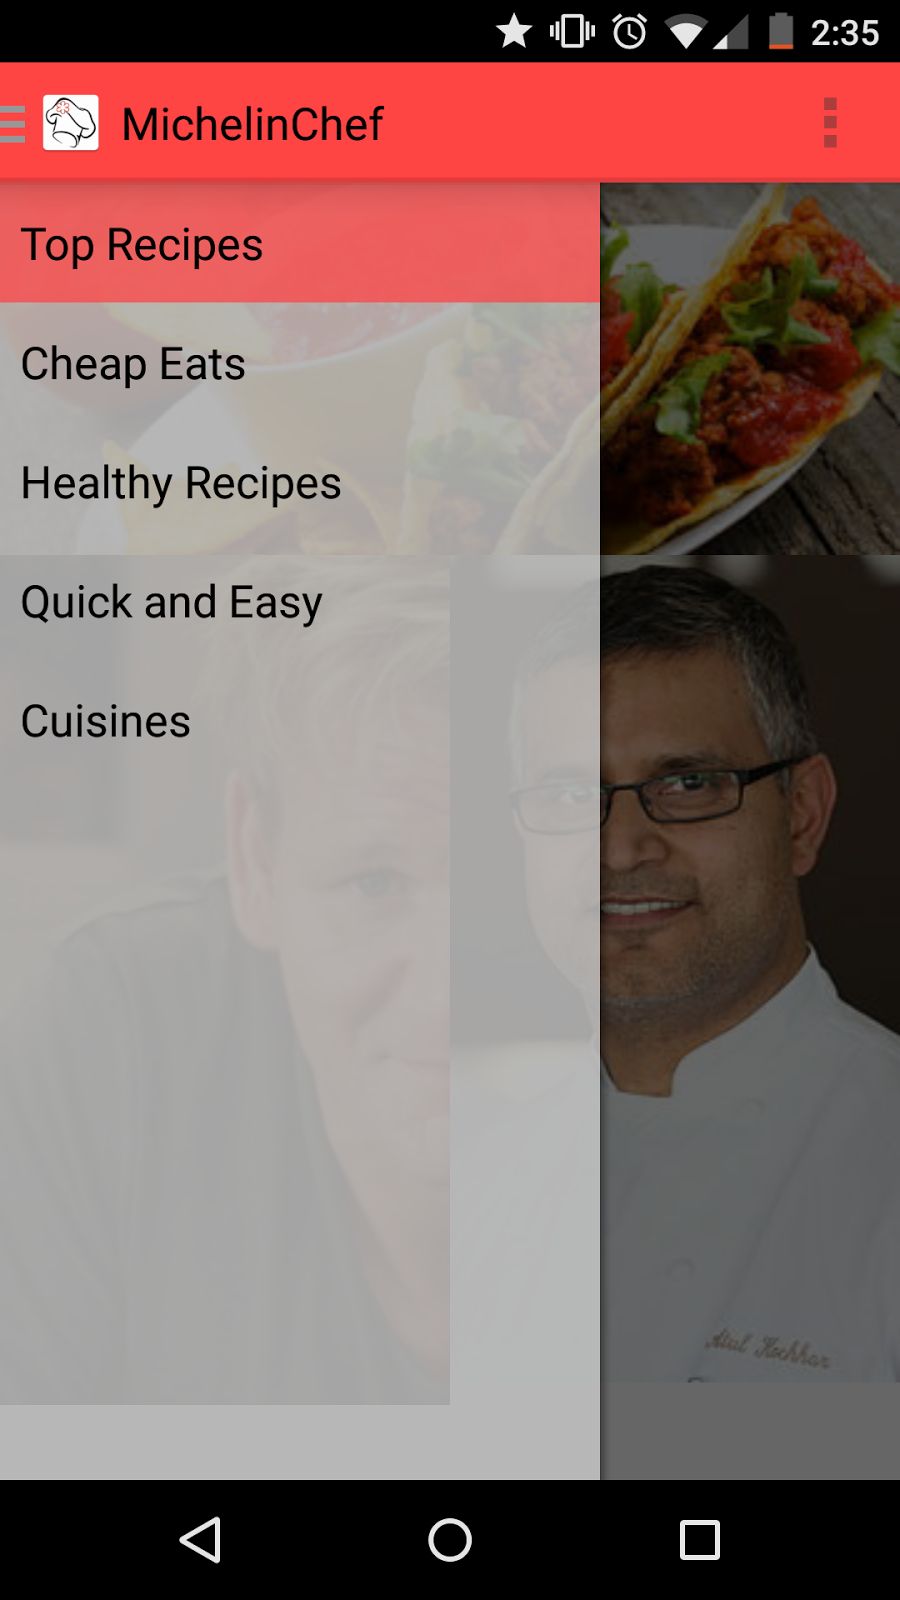
\includegraphics[width=0.3\textwidth, height=0.3\textheight]{images/nav_draw.png}
	\caption{Navigation Drawer to access the different categories of menus\label{fig_1}}
\end{figure}

\begin{figure}[ht!]
	\centering
	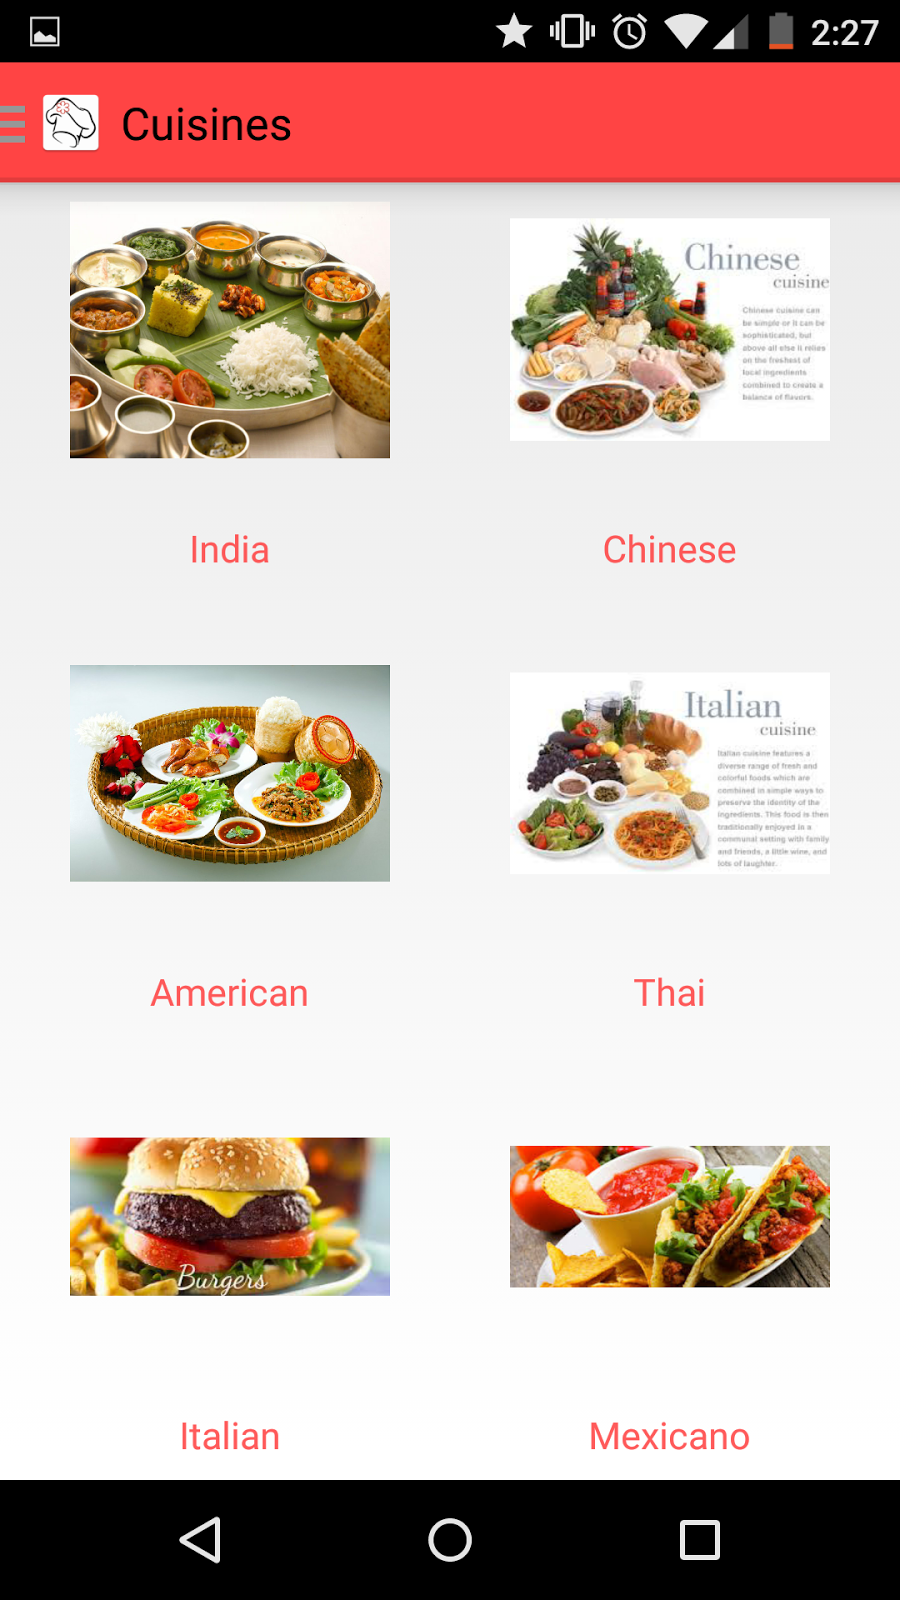
\includegraphics[width=0.3\textwidth, height=0.3\textheight]{images/cuisines.png}
	\caption{Origin based categorization of cuisines\label{fig_2}}
\end{figure}

\begin{figure}[ht!]
	\centering
	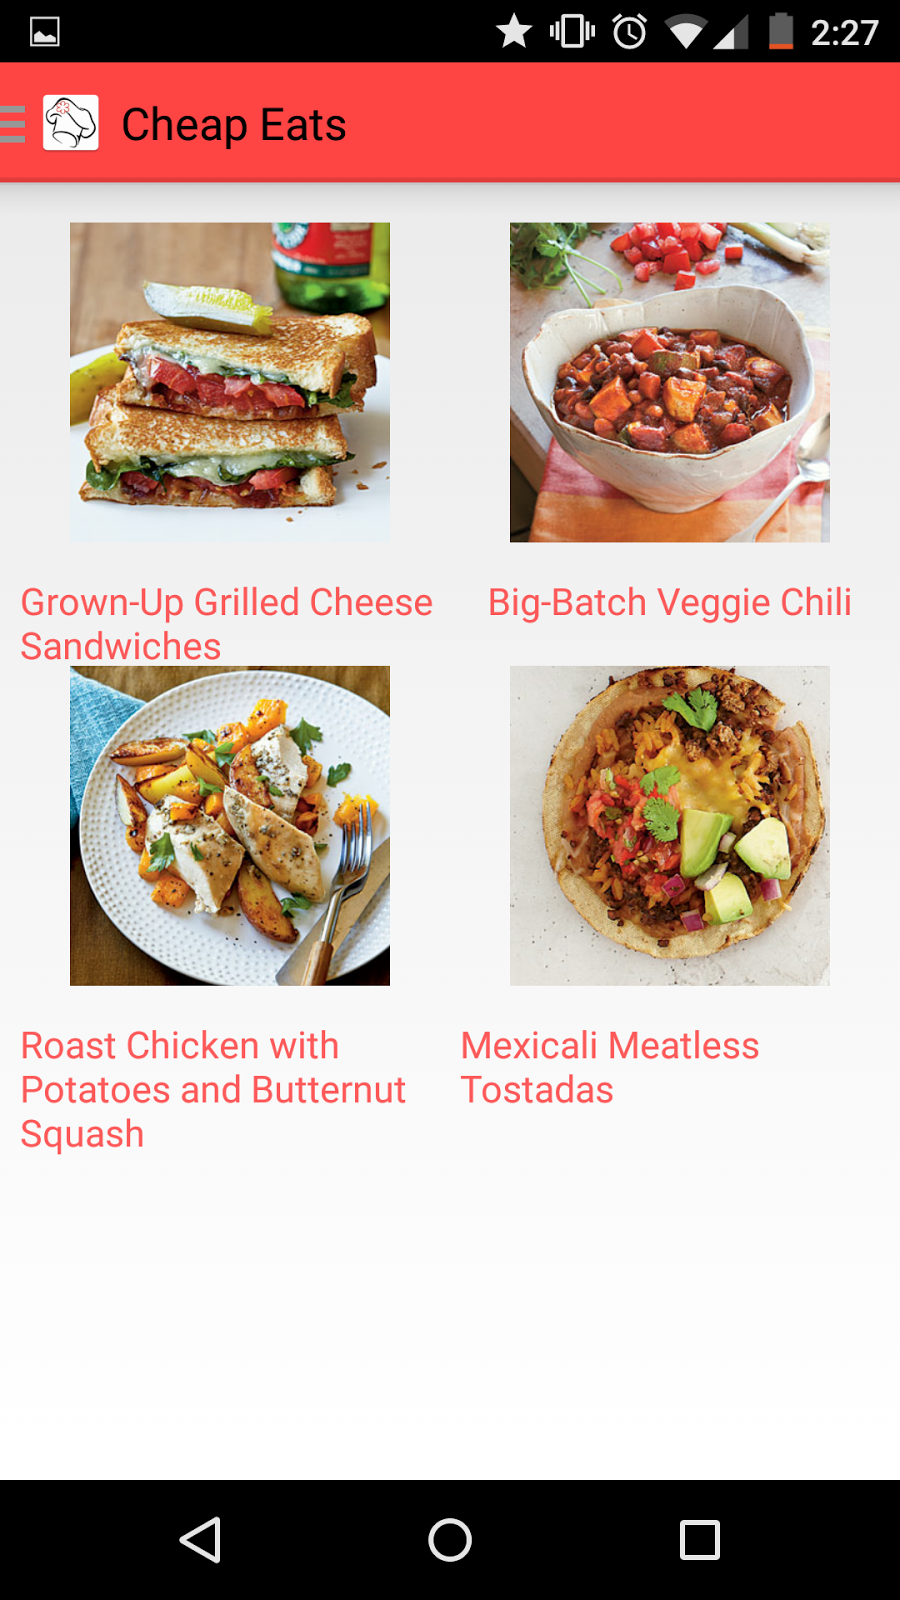
\includegraphics[width=0.3\textwidth, height=0.3\textheight]{images/cheap_eats.png}
	\caption{Different categories of recipes - Cheap Eats\label{fig_3}}
\end{figure}

\begin{figure}[ht!]
	\centering
	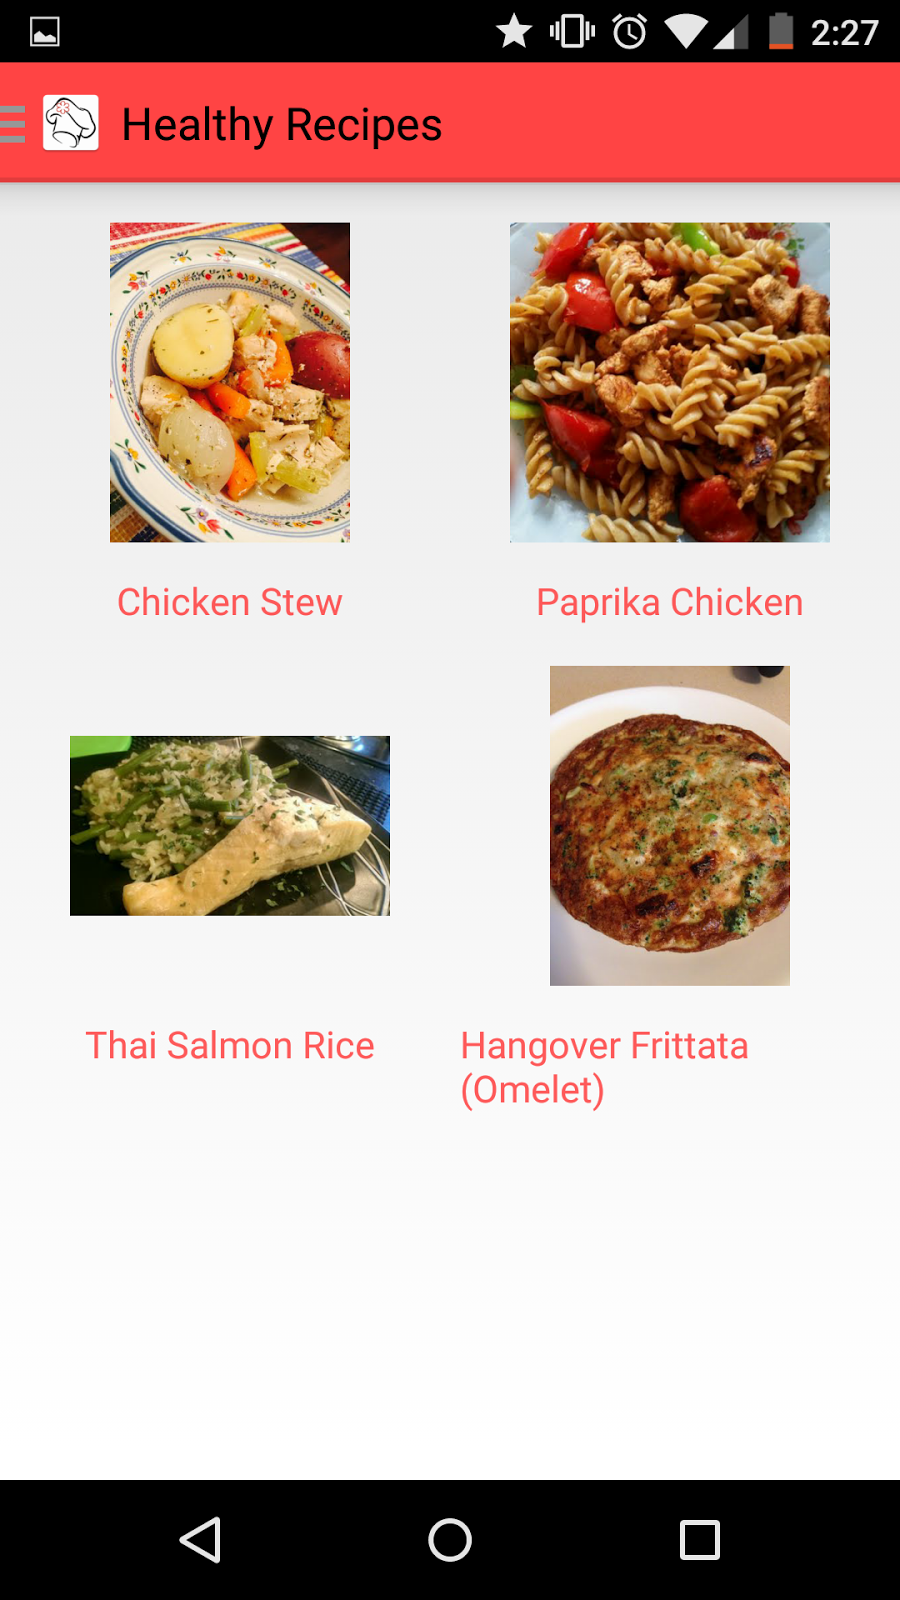
\includegraphics[width=0.3\textwidth, height=0.3\textheight]{images/healthy.png}
	\caption{Different categories of recipes - Healthy\label{fig_4}}
\end{figure}

\begin{figure}[ht!]
	\centering
	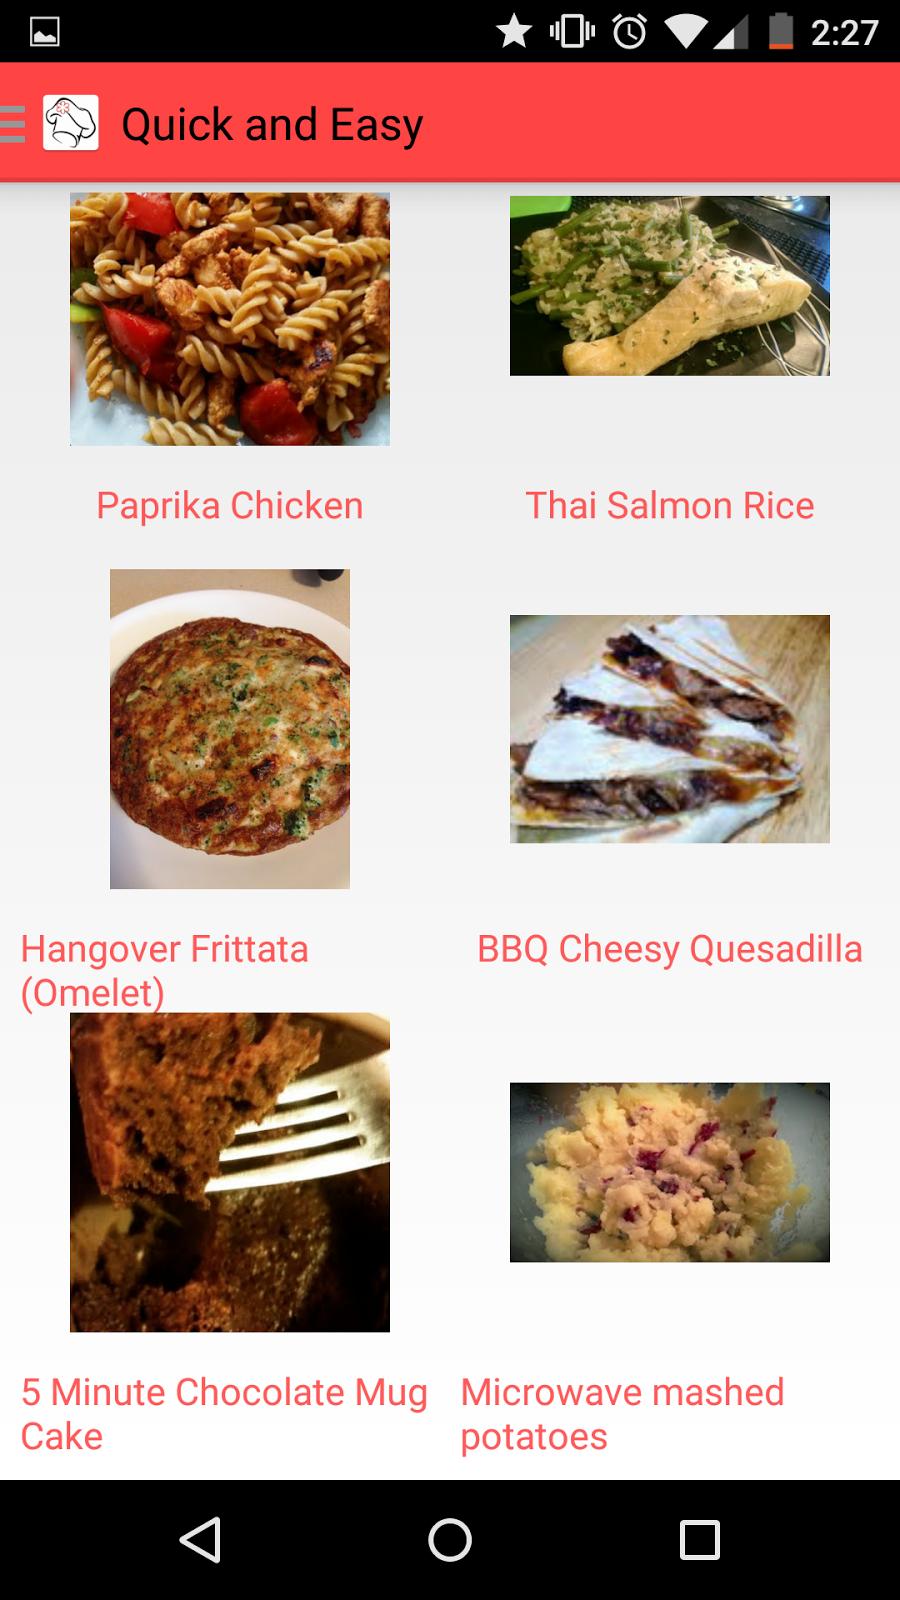
\includegraphics[width=0.3\textwidth, height=0.3\textheight]{images/quick_easy.png}
	\caption{Different categories of recipes - Quick \& Easy\label{fig_5}}
\end{figure}


\begin{figure}[ht!]
	\centering
	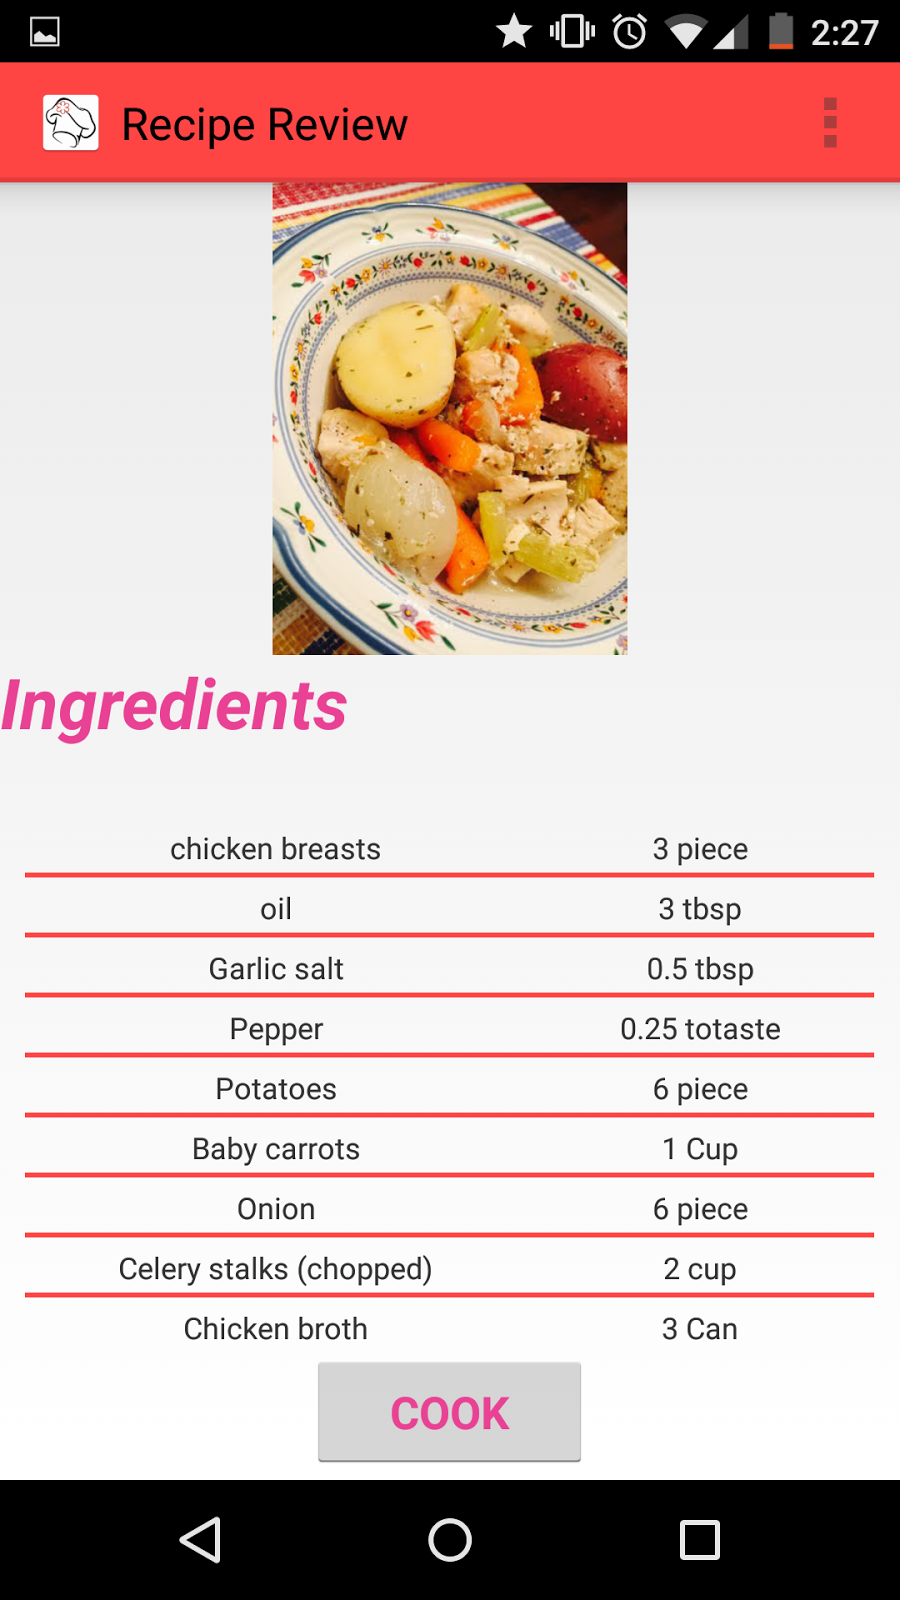
\includegraphics[width=0.3\textwidth, height=0.3\textheight]{images/recipe_review.png}
	\caption{Recipe Review screen that shows the ingredients \label{recipe-review}}
\end{figure}


\begin{figure}[ht!]
	\centering
	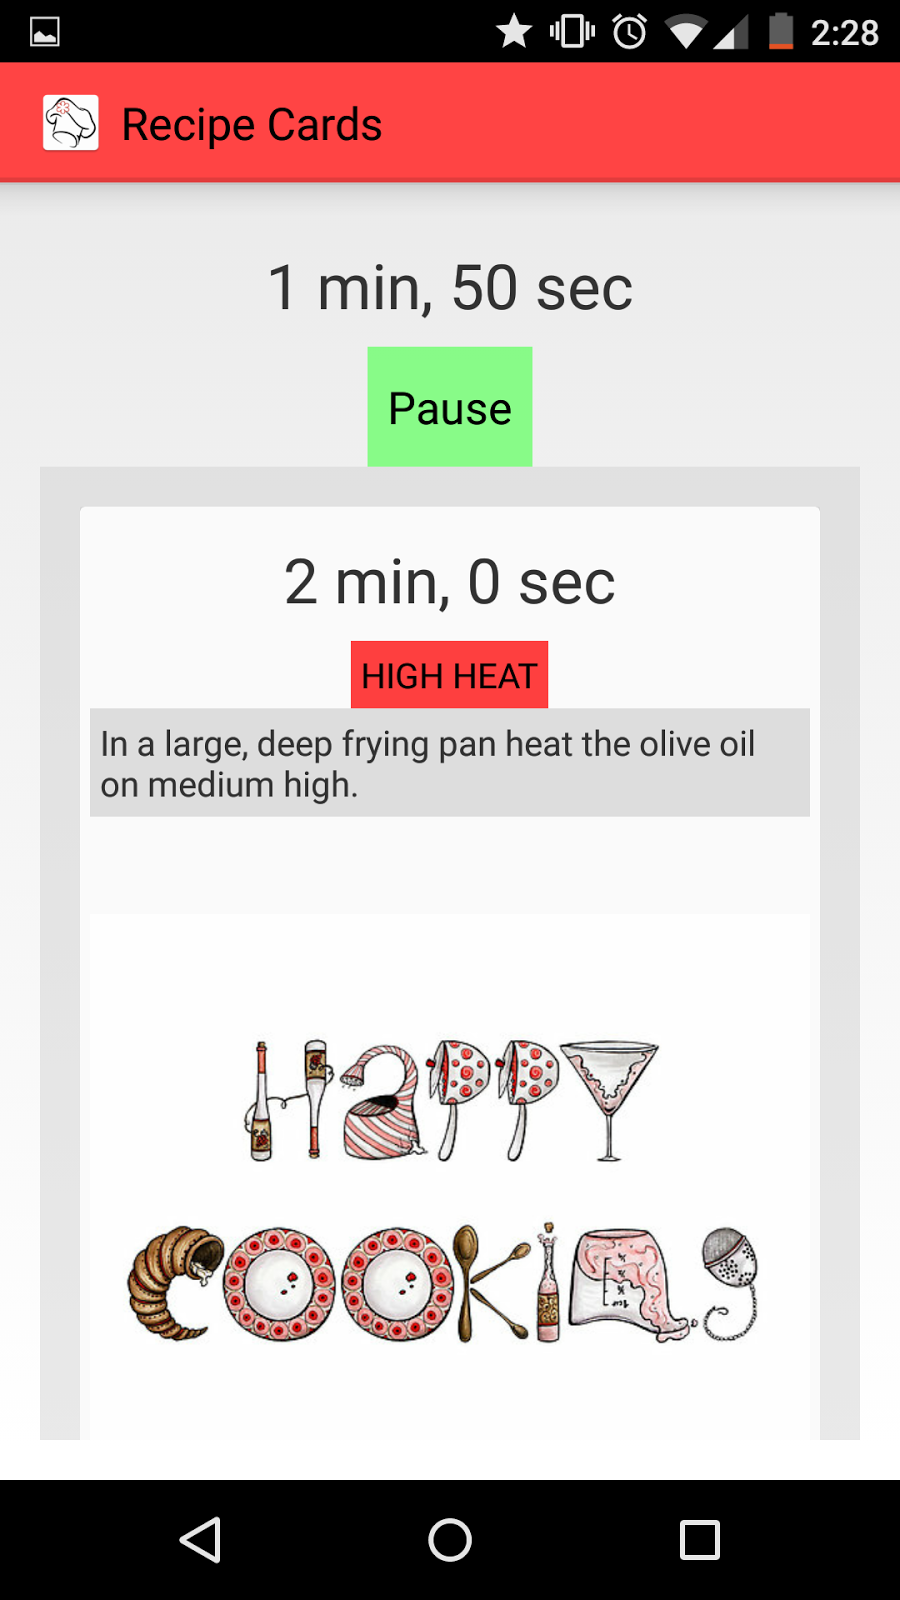
\includegraphics[width=0.3\textwidth, height=0.3\textheight]{images/recipe_cards_1.png}
	\caption{Recipe card that enables easy delivery of cooking instructions \label{recipe-card1}}
\end{figure}

\begin{figure}[ht!]
	\centering
	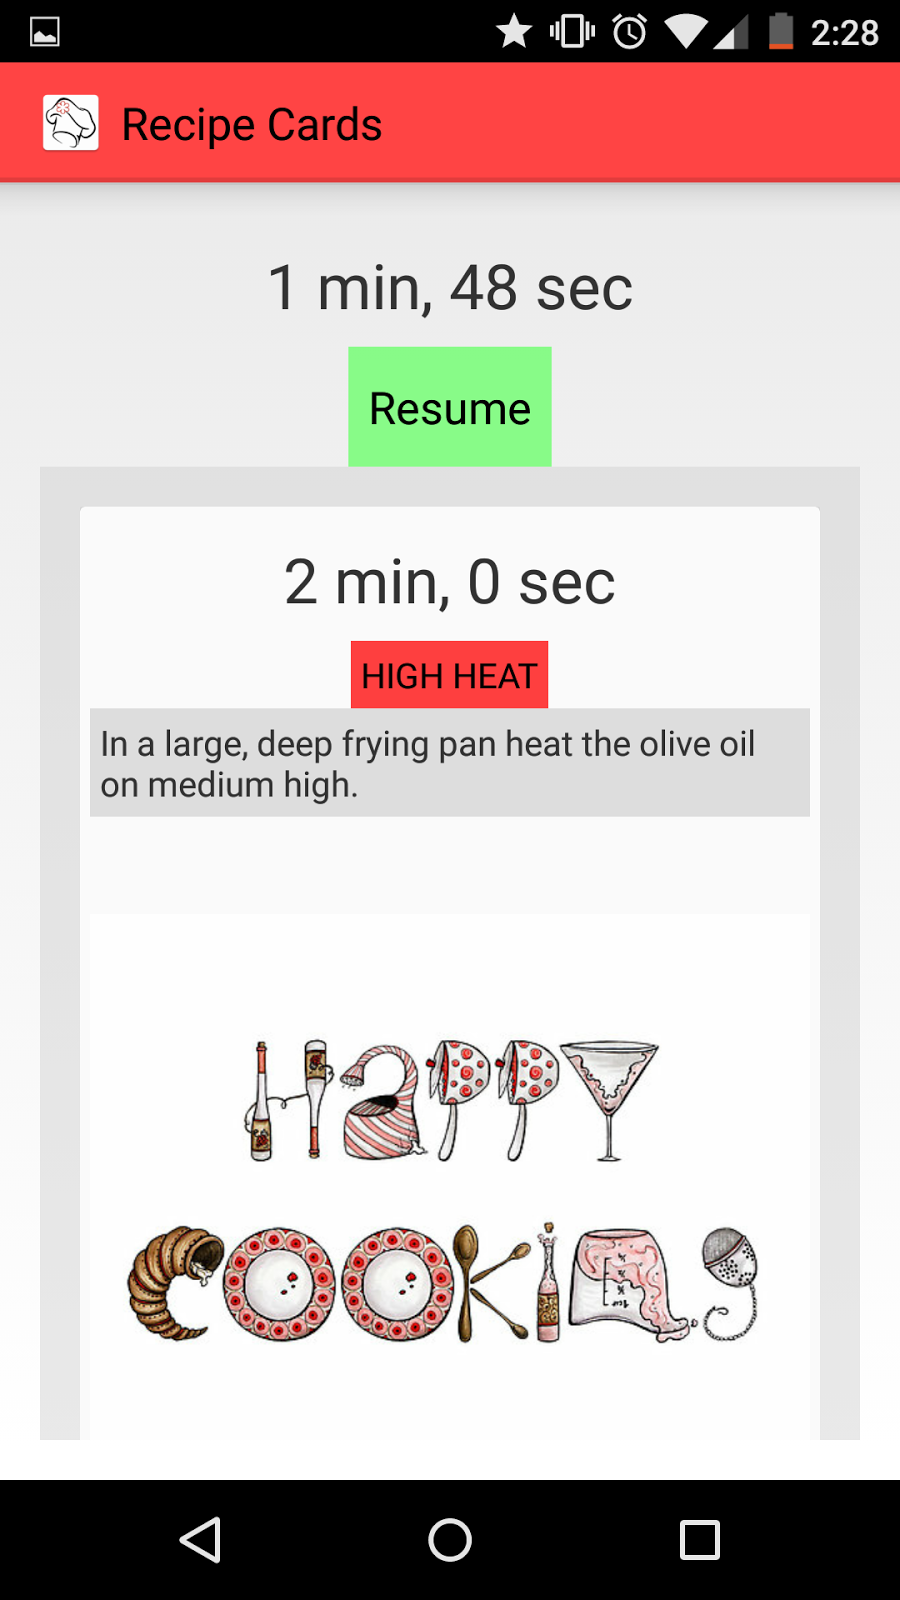
\includegraphics[width=0.3\textwidth, height=0.3\textheight]{images/recipe_cards_2.png}
	\caption{Recipe card that enables easy delivery of cooking instructions \label{recipe-card2}}
\end{figure}

\subsection{Step 2 : Android Implementation}
Following our UI prototyping, we implemented our app using Android Lollipop 5.0 SDK 
\cite{lollipop}. 
In our implementation we used Android framework components such as Fragments \cite
{fragments} and activities \cite{activites}. 
We implemented the following functionality in the app 
\begin{itemize}
\item Different categorization of recipes
\item Recipe review and recipe cards \cite{CardView} for each recipe
\end{itemize}
We implemented two different categorizations 
\begin{enumerate}
\item Quality of food based categorization viz
	\begin{enumerate}
		\item Cheap Eats recipes
        \item Quick and Easy recipes
        \item Healthy food recipes
	\end{enumerate}
\item Origin based categorization viz
	\begin{enumerate}
		\item Indian,
        \item Chinese,
        \item American,
        \item Mexican etc... 
	\end{enumerate}
\end{enumerate}

In order to allow for reuse and to keep the app light on memory consumption, we built all categories over fragments.
A fragment is a reusable part of the application for often re-occurring structures. 
Since the quality of food categories are very similar, we built fragments for each of them and dynamically replace fragments according to user input. 
In order to make navigation as efficient as possible, we built a navigation drawer layout - a structure that launches user action menus by the swipe from the left end of the user interface.
Each of the fragments were tied to this navigation menu.
We also implemented the origin based categorization in a similar fragment.

We also implemented the recipe review screen for each recipe. 
The recipe review screen takes a given recipe as input and displays the end image and the ingredients that are needed. 
The ingredients are taken from the database and are displayed in a user-friendly manner (table).
After reviewing the recipe ingredients, the chef can click on the 'Cook' button. 
Once it is clicked, the digital cards are displayed to the user.
The user can review all the steps required for the recipe and read through the entire layout once if he so desires.
Once the chef is ready to cook, he may click the 'Start' button and the timer starts.
Each step of the recipe has a timer associated with it. When the user clicks the 'Start' button, the first step timer is fired and is counted down. Once it is complete, the step is removed from user view (via scrolling) and the next step is shown and the next step's timer is now fired. 
This is repeated for all steps until the last step. Once all the timers run out, the recipe is completed. In addition, the chef is allowed to pause/resume the flow of cards according to his/her will.

\subsection{Step 3: Database Implementation}

\begin{figure*}[ht!]
	\centering
	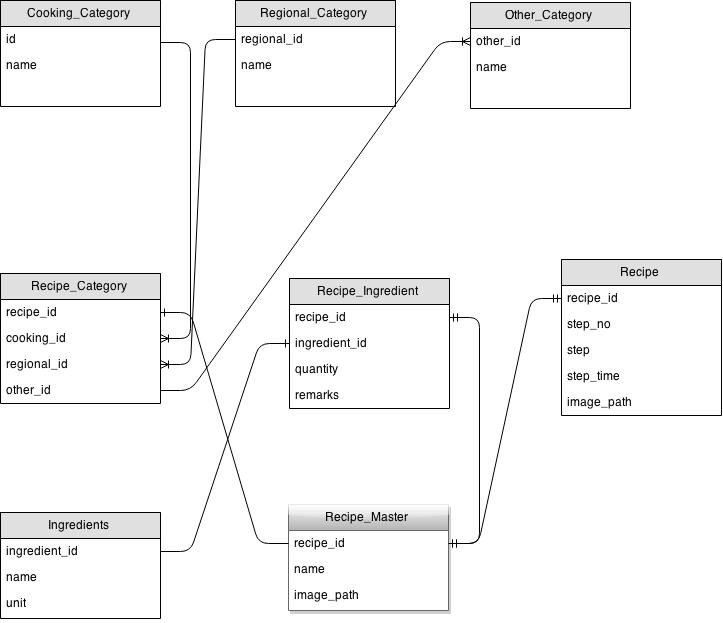
\includegraphics[width=0.8\textwidth, height=0.4\textheight]{images/db.jpg}
	\caption{Database scheme \label{db-schema}}
\end{figure*}

We have used Android SQLite database for this application. SQLite is a very light weight database which comes with Android OS. Basic Database design for the application is as follows (and shown in Figure \ref{db-schema}).

\begin{enumerate}
\item Cooking\_Category : This is a master table for recipe categories based on cooking method. It contains category id and name where id is the primary key.	


\item Regional\_Category :  This is a master table for recipe categories based on regional origin of the recipe. It contains regional category id and name where id is the primary key. 
\item Other\_Category : This is a master table for other recipe categories such as Quick \& Easy, Cheap eats or Healthy Recipes. It contains category id and name where id is the primary key. 
\item Ingredients : This table contains all the ingredients for all of the recipes inside database. This table contains id, name and quantity unit of the ingredient where id is the primary key.
\item Recipe\_Master : Recipe\_Master table is master table where all the recipes, their ids and display image paths are stored. Recipe\_id is the primary key of this table.
\item Recipe\_Category : This table contains information about which recipe belongs to which category. It contains recipe\_id, cooking\_id, regional\_id and other\_id which all are Foreign keys of Recipe\_Master, Cooking\_Category, Regional\_Category and Other\_Category tables respectively.
\item Recipe\_Ingredients : This table contains list of ingredients for each recipe along with quantity and any other remarks. recipe\_id and ingredient\_id are the foreign keys from Recipe\_Master and Ingredients tables respectively.
\item Recipe : This table contains all the steps required to perform cooking with step number, step time and image (if available) for each step. Recipe\_id is the foreign key from Recipe\_Master table.
\end{enumerate}

\subsection{Database Integration with the Application}
Once the database was implemented, we integrated our application with it using Android SQLite APIs. We populated our user interface with data read from Database using Database Helper class. In Database Helper class, we have implemented different helper methods that execute SQL queries using rawQuery API of SQLite and retrieve the appropriate recipe data and pass it on our Android activities. 

Recipe categories implemented as Android Fragments such as Cuisines, Quick and Easy, Cheap Eats, Healthy calls their corresponding Database Helper methods. They return data back to these Categories. Once the recipe category fragments receive data from database helper methods they show the content such as recipe text and recipe image to the user. 

When the user clicks one of the dishes, the recipe category Fragment passes the Recipe ID as part of intent object to the Recipe Preview screen activity. The Recipe preview screen activity after retrieving the Recipe ID from the intent object calls Database Helper method with the Recipe ID to retrieve the appropriate list of ingredients and their quantities and Recipe Image on the Recipe preview screen. 

After the user reviews the recipe review screen and decides to cook that dish, they will click the 'Cook' button. When that happens, the same intent bounded with Recipe ID will be passed to Recipe Digital Card activity. Similar to the Recipe preview screen, Recipe Digital card activity retrieves List of recipe steps, time required for each of the recipe steps, Images required for each of the recipe steps from the Database Helper class by passing on the Recipe ID . Essentially, Database helper uses Recipe ID and executes the SQL query on database to get the corresponding results.

\subsection{Step 4: Hardware System Design}
This is an embedded system made up of a cook-top \cite{cook-top}, \cite{cook-top1}, a microcontroller with a Temperature sensor and a Bluetooth module.

\begin{figure*}[ht!]
	\centering
	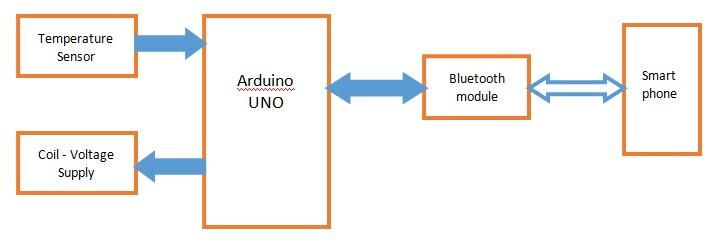
\includegraphics[width=0.8\textwidth, height=0.2\textheight]{images/hw_1.jpg}
	\caption{Top Level design of Smart Cook-Top \label{hw_1}}
\end{figure*}

\begin{figure*}[ht!]
	\centering
	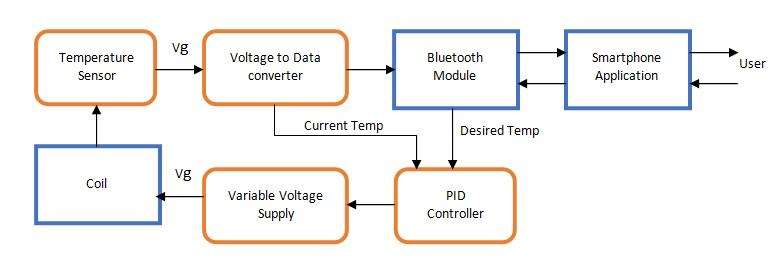
\includegraphics[width=0.8\textwidth, height=0.2\textheight]{images/hw_2.jpg}
	\caption{Data flow model of Smart Cook-Top design \label{hw_2}}
\end{figure*}

The temperature sensor senses the current temperature of the coil and then sends this data in the form of an analog signal(voltage signal ~10mv). The arduino reads the voltage level on the analog input pin available on the board. The voltage level is processed in the arduino and the equivalent temperature information is sent on the serial communication lines to the bluetooth module, this temperature information is then wirelessly transmitted to the paired smartphone. The temperature value can be viewed on MichelinCook.

The desired temperature value of the cook-top is sent from the MichelinCook application to the bluetooth module which is then sent to the arduino module. To set the cook-top to a particular temperature, a PID algorithm is implemented in the arduino, it makes use of the current temperature and the desired temperature values to calculate the required change in the voltage value. The new voltage is supplied to change the temperature in steps till the desired value of temperature is reached. 

The smart cook-top to control temperature and communicate with MichelinCook application was prototyped in simulink. The simulink model was used to simulate the design to check for its working and functionality.

% \begin{figure}[ht!]
% 	\centering
% 	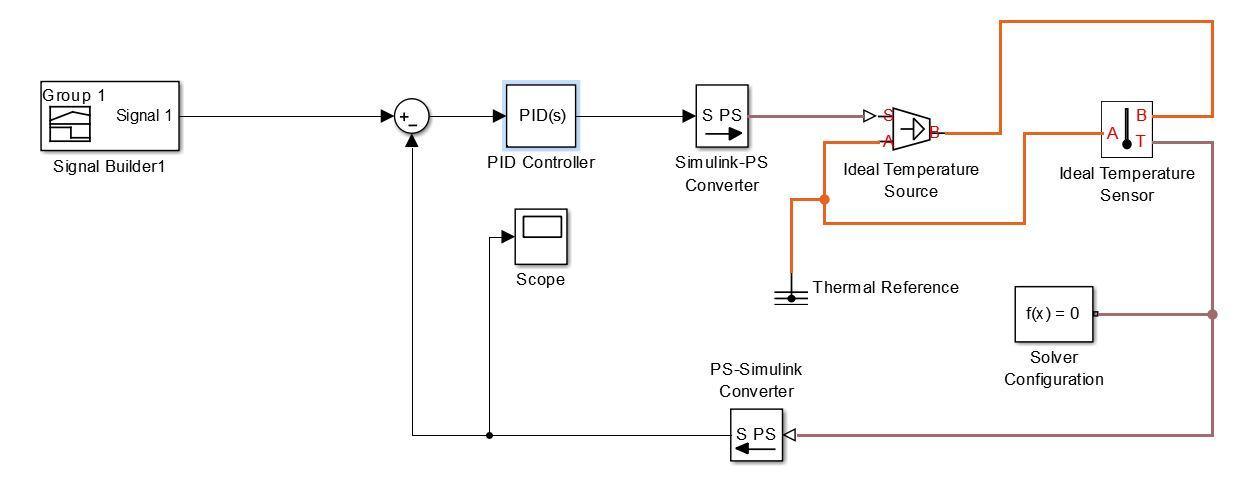
\includegraphics[width=0.4\textwidth, height=0.2\textheight]{images/hw_3.jpg}
% 	\caption{Data flow model of Smart Cook-Top design \label{hw_2}}
% \end{figure}

The signal builder in Fig 13 is configured to present temperature values relative to time. The signal builder has temperature values of 80C from 0s to 300s and 100C from 300s to 1000s. The cook-top coil is modelled as an Ideal temperature source in this phase of the project. The closed system has a PID controller which is a commonly used controller in industries.

The PID values are selected to minimize the rise and have low overshoot as possible. The output of the closed loop system is monitored using the scope. The signal waveform corresponding to input signal from signal builder and output temperature as sensed by the temperature sensor is as shown in figure below.

% \begin{figure*}[ht!]
% 	\centering
% 	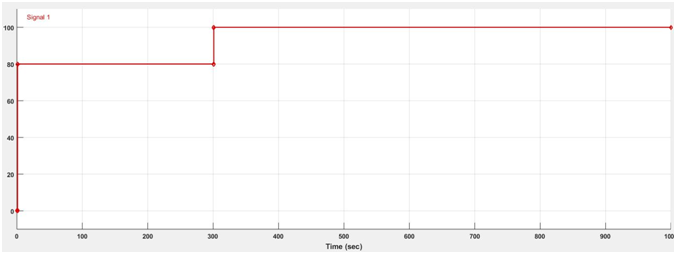
\includegraphics[width=0.8\textwidth, height=0.2\textheight]{images/hw_4.png}
% 	\caption{Output signal given the input signal \label{hw_4}}
% \end{figure*}

% \begin{figure*}[ht!]
% 	\centering
% 	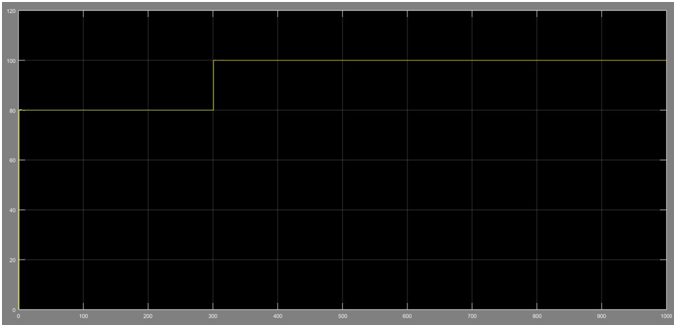
\includegraphics[width=0.8\textwidth, height=0.2\textheight]{images/hw_5.png}
% 	\caption{Mathematical response for real cook-top process\label{hw_5}}
% \end{figure*}

To develop the mathematical response for the real [non ideal] cook-top process is very important. Most processes similar to cook-tops are modelled using First or Second order plus dead time models.

\begin{figure*}[ht!]
	\centering
	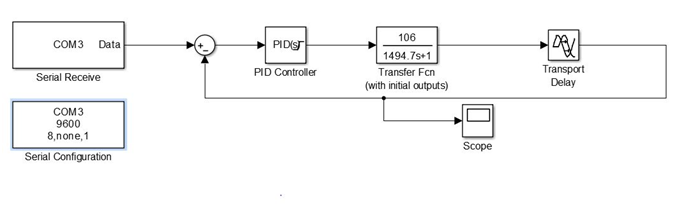
\includegraphics[width=0.8\textwidth, height=0.2\textheight]{images/hw_6.png}
	\caption{Real Cook-Top Design with real cook-top behavior modelled using FODPT \label{hw_6}}
\end{figure*}

\begin{figure*}[ht!]
	\centering
	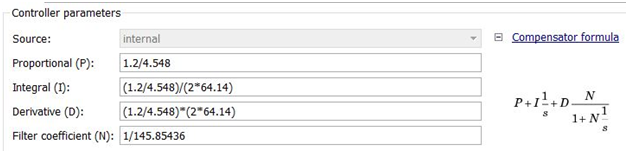
\includegraphics[width=0.8\textwidth, height=0.2\textheight]{images/hw_7.png}
	\caption{PID parameters \label{hw_7}}
\end{figure*}

The response graph for the real cook-top is as shown in the figure below.

% \begin{figure*}[ht!]
% 	\centering
% 	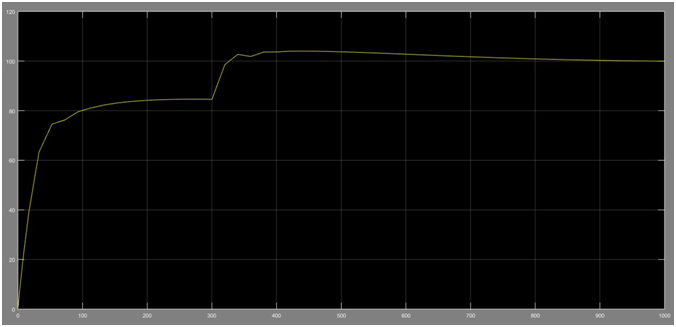
\includegraphics[width=0.8\textwidth, height=0.2\textheight]{images/hw_8.png}
% 	\caption{Temperature response of real(FODPT) cook-top coil \label{hw_8}}
% \end{figure*}









\section{Evaluation}

We used Lean Startup \cite{LeanStartup} model for evaluation of our mobile application idea. The advantage of using Lean Startup Methodology in mobile development includes,
\begin{itemize}
	\item Faster time to market
	\item Lower Cost Overall and Upfront Cost
	\item Less Financial Risk
	\item Build a Better product that customers want.
	\item Less wasted time
\end{itemize}

In our case as this is a course project, the most relevant use of Lean Startup Methodology is for building a better product that customer wants and with a shorter design cycle time.

\subsection{Building an MVP}
A minimum viable product \cite{MVP} is a product with only the core features. We plan to use the current version of  our application as MVP for the purpose of testing. The MVP will be deployed for testing among early adopters whose feedback will be collected for further enhancement of the application.

The MVP is a way to test with the objective of answering four questions:
\begin{itemize}
	\item Do users recognize that they have the problem we are trying to solve?
	\item If there is a solution, would they use it?
	\item Would they use our app?
	\item Are we building a solution for the above problem?
\end{itemize}

If the answer is yes for four of the above questions, then we have an actual requirement for such an application. Building an MVP is a way to collect feedback, user response, and test the waters. The challenge of building an MVP can be a bit more difficult on mobile. There is a higher bar for mobile applications. We have to be a bit more refined as people are less patient on mobile and there is a much lower tolerance for bugs.


\subsection{User Feedback}
Each feature built are like experiments to see how users adopt and engage in the product. In the early stage of building a product, it is extremely important to talk to your customers. The early adopters, beta testers, and evangelists are key for customer discovery. We need to evaluate if our core proposed product features solve their problem. Data gathered from the first group of beta users will be key for figuring out what features to focus on.

\subsection{Quantitative and Qualitative Metrics}
The feedback from users are extremely useful and comes in both qualitative and quantitative forms. There are certain key metrics to focus on that will demonstrate health. One of the most important focus for our application is to measure engagement. Nothing signals stickiness and that you have something with your MVP than to have good engagement in your app. Some hard metrics that shows engagement in mobile includes:
\begin{itemize}
	\item Active Users : Number of active users a day/week/month is essential for measuring
	\item Session Length : How long do the users spend in your app. The time they open to the time its closed.
	\item Session Interval : How long in between each session of usage
	\item Screen Flow : Interactions in the app between each screens, duration on each screens, and the total number of occurrences in each screen.
	\item Retention Rate : the percentage of users who return to the app based on the date of their first visit.
\end{itemize}

In addition to these quantitative forms of measuring engagement, it is also important to observe and watch users engage in our app for UX purposes.  Direct communication from users may be best for clear feedback of the app.

Any user data points gathered, both qualitative and quantitative, can be extremely beneficial  for a glance at user behavior to learn and provide direction for app development. It is crucial to track user behavior, feedback, and use the information when building new features.

\section{Future Work}

In this section, we discuss our future work from following perspectives: implementation, functionality and user experience.

\subsection{Implementation}
Currently we only implement ''MichelinCook'' on Android system. In the future, we also plan to implement it on iOS, which is also one of the most popular smartphone system. And we also plan to upload our app to both Android Market and iOS App Market.

\subsection{Functionality}
Self-timed digital card is very helpful for cooking. However, it needs users to manually pause/resume the cards. In the future, we may add voice control so that users can cook the dish without ever having to click the app.

In addition, we plan to add functions to allow the user to upload their own recipes and some happen-before  relations (e.g.,  step 1 should go first than another step 2) for  their recipes. Our app can then automatically generate the optimized step sequence with corresponding time card.

\subsection{User experience}
We plan to make a survey of our app among other students and ask some feedback about the current interface, functions and features. Using their feedback we can add more new functions and features.
\section{Conclusion}

Cooking is an integral part of a person's life and it is folk-wisdom that the best way to reach a man's heart is through his stomach. But cooking becomes a challenging task if the user is inexperienced or when trying new recipes. We conducted a short survey of existing recipe delivery mechanisms and found that they're clumsy and not ideal solution for cooking. Most of these mechanisms require human intervention to get through each and every step of the recipe - this would make each of them very inconvenient to use. 

We solved this problem by providing a new mechanism of recipe delivery - digital cards. A card is shown for each step of the recipe and the card contains instructions as to what that step is and an image accompanying the outcome of that step. Each card has a timer which counts down and on expiry the card moves on to the next card containing the next step of the recipe. This automatic navigation to different steps makes MichelinCook a very convenient tool to use in one's kitchen. Our evaluation techniques have also confirmed our hypothesis and we plan to release the application on the Android Play Store very soon.
\begin{thebibliography}{50}

\bibitem{CardView} CardView | Android Developers  [Online] May 2015. Available: https://developer.android.com/reference/\\android/support/v7/widget/CardView.html

\bibitem{lollipop} Android - 5.0 Lollipop [Online] May 2015. Available: https://www.android.com/intl/\\en\_us/versions/lollipop-5-0/

\bibitem {fragments} Fragments | Android Developers  [Online] May 2015. Available: http://developer.android.com/guide/components\\/fragments.html

\bibitem {activites} Activites | Android Developers  [Online] May 2015. Available: http://developer.android.com/guide/components\\/activities.html

\bibitem{LeanStartup} The Lean Startup | Methodology [Online] May 2015. Available: http://theleanstartup.com/principles

\bibitem{MVP} The Lean Startup | Methodology [Online] May 2015. Available:
http://theleanstartup.com/principles

\bibitem{cook-top} D. Ding, R. A. Cooper, P. F. Pasquina, and L. Fici-Pasquina, ''Sensor technology for smart homes,'' Maturitas, vol. 69, no. 2, pp. 131 - 136, 2011.

\bibitem{cook-top1} S.R. Patil, Raveena Chavan, ''Intelligent Cooking Providing Automatic Time and Temperature Setting Using Image Processing With Wide Range of Recipes for Microwave Ovens'', Department of Computer Engineering, Pune University, Pune, India. received on December, 2013.

% \bibitem{MichelinCook} Murcott,A.(1983) ''Women's Place: CookBook's images of technique and technology in the British Kitchen'',Women's Studies International forum,Vol.6,No.1,pp.33-9.

\end{thebibliography}
\section*{Acknowledgment}
We thank all group members for working hard on getting the project together. We also would like to thank Dr. Shipman for providing us guidance throughout the semester.


% That's all folks!
\end{document}